%%%%%%%%%%%%%%%%%%%%%%%%%%%%%%%%%%%%%%%%%%%%%%%%%%%%%%%%%%%%%%%%%%%%%%%%%%%%%%%%
%2345678901234567890123456789012345678901234567890123456789012345678901234567890
%        1         2         3         4         5         6         7         8

\documentclass[letterpaper, 10 pt, conference]{ieeeconf}  % Comment this line out if you need a4paper
\usepackage{graphicx}
\usepackage{subcaption}
\usepackage{cite}
\usepackage{multicol}
\usepackage{url}
\usepackage{textcomp}
\usepackage{textgreek}
\usepackage{fixltx2e}


%\documentclass[a4paper, 10pt, conference]{ieeeconf}      % Use this line for a4 paper

\IEEEoverridecommandlockouts                              % This command is only needed if 
                                                          % you want to use the \thanks command

\overrideIEEEmargins                                      % Needed to meet printer requirements.

% See the \addtolength command later in the file to balance the column lengths
% on the last page of the document

% The following packages can be found on http:\\www.ctan.org
%\usepackage{graphics} % for pdf, bitmapped graphics files
%\usepackage{epsfig} % for postscript graphics files
%\usepackage{mathptmx} % assumes new font selection scheme installed
%\usepackage{times} % assumes new font selection scheme installed
%\usepackage{amsmath} % assumes amsmath package installed
%\usepackage{amssymb}  % assumes amsmath package installed

\title{\LARGE \bf
Cycloidal Geartrain In-Use Efficiency Study
}

\author{Logan C. Farrell$^{1}$, James Holley$^{2}$, William Bluethmann$^{3}$, and Marcia K. O'Malley$^{4}$% <-this % stops a space
\thanks{$^{1}$Logan Farrell is with the Department of Mechanical Engineering at Rice University and NASA: Johnson Space Center.
		{\tt\small Logan.C.Farrell@NASA.gov}}%
\thanks{$^{2}$James Holley is with the Department of Mechanical Engineering at Rice University and NASA: Johnson Space Center.}%
\thanks{$^{3}$William Bluethmann is the project manager for rovers at NASA: Johnson Space Center.}%
\thanks{$^{4}$Marcia O'Malley is on the Faculty in the Department of Mechanical Engineering at Rice University, Houston, TX}%
}


\begin{document}

\maketitle
\thispagestyle{empty}
\pagestyle{empty}

\begin{abstract}
Currently, harmonic drives are the primary speed reducer for robotic applications where a high reduction in a small package is required. 
Cycloidal drives are an alternative option for high reduction, small package, use-cases with the advantage of a higher specific torque and the ability to customize and integrate the drive for the application.
These compact style cycloidal drives have been well studied in theory and simulation for their performance, but very little data is available on their actual performance over time. 
This paper presents experimental data on performance of a cycloidal drive designed for a robotic application. 
Burn-in time efficiency curves and torque/speed efficiency profiles are computed after running the drive through 51k output cycles (3M input cycles) over the course of 111 hours of testing. 
The study finds that substantial burn-in time may be required for steady-state performance, but peak efficiencies of 80\% can be achieved. 
Also, the efficiency is shown to be dependant on the torque through the actuator.
This work demonstrates a customized cycloidal drive in a robotic application that is comparable to a harmonic drive in efficiency performance, with a 2x increase in specific torque, suggesting the application of cycloidal drives could grow tremendously in robotic designs. 
\end{abstract}

\section{Introduction}
\label{intro}
As robotic applications flourish in our modern world, there is an increasing need for high reduction, high torque, and low backlash actuator systems.
These actuators are present in all types of robotic equipment and are critical in space flight applications.
A notable recent example includes the Curiosity rover from NASA's Jet Propulsion Laboratory that uses 33 separate motors with various reductions \cite{curiosity}.
Currently, harmonic drives are the primary reduction method when high ratio and compact design are required.
Commercially, these reducers come in limited reduction ratio options, and require a substantial amount of additional mass to withstand high torque applications.
Ideally, one would be able to specify a desired reduction ratio and realize it in a compact, lightweight package. 
Cycloidal drives are potentially an apt replacement for these harmonic drives as they can offer a large reduction in a small package.

\begin{figure*}[t]
	\centering
	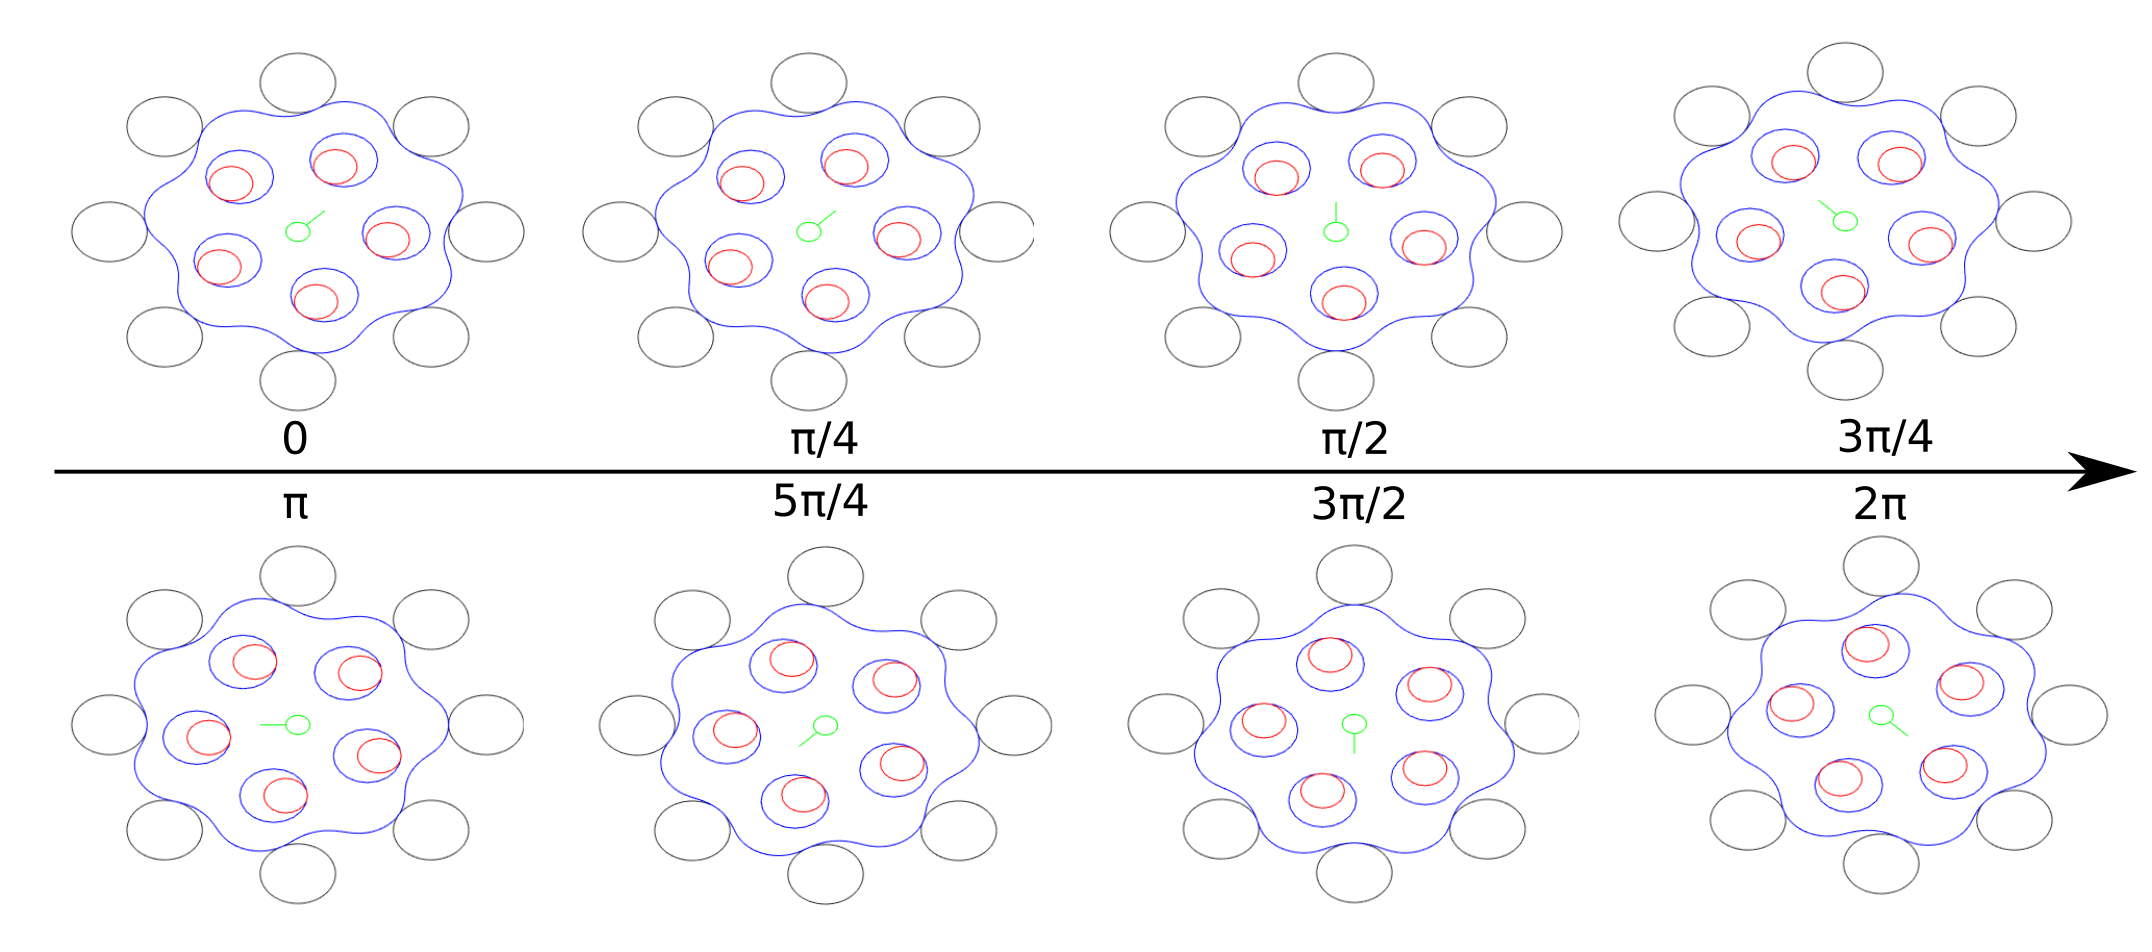
\includegraphics[width=0.8\linewidth]{images/single_motion}
	\caption{An example of a cycloid actuators motion with eight housing pins (black), seven lobes (blue) for a ratio of 7:1 and fie output pins (red). A single input revolution of the green input shaft is shown, resulting in 1/7 counter-rotation of the cycloid plate. This counter-rotation presses against the red pins, resulting in the output counter-rotation. 
	}
	\label{cycloid_motion}
\end{figure*}


\subsection{Cycloidal Drive Motivation}

Cycloidal drives cheive reductions that would require three or more stages in a tradiational planeatry drive. 
In situations where small backlash is acceptable, generally less than 1 arc-min, cycloids offer distinct advantages.

\begin{enumerate}
\item
Cycloids can be customized into the system directly. They allow specific reductions and load selection and can be incorporated directly into the actuator housing.
\item
Cycloids are made of relatively easy to manufacture parts compared to a harmonic drive.
\item
The torque to weight ratio is typically higher for cycloidal drives of this style over a harmonic drive.
For example, the cycloid presented in this work is 2.5kg including all housing components, while a comparable harmonic drive is 5.1kg.
\end{enumerate}

Cycloidal drives have many desirable characteristics. These characteristics are covered well on a theoretical basis in the literature. However, these actuators are not commonly used in robotic actuator design, potentially due to the lack of in-use operational data to verify the theoretical analysis.

The primary contribution of this research is to quantify the efficiency of a cycloidal drive system through an extended drive cycle test for burn-in to steady state performance and efficiency over the torque/speed profile.
To date, the actuator has been subjected to over 129k output revolutions through over 300 hours.

\begin{figure}[!b]
   \centering
   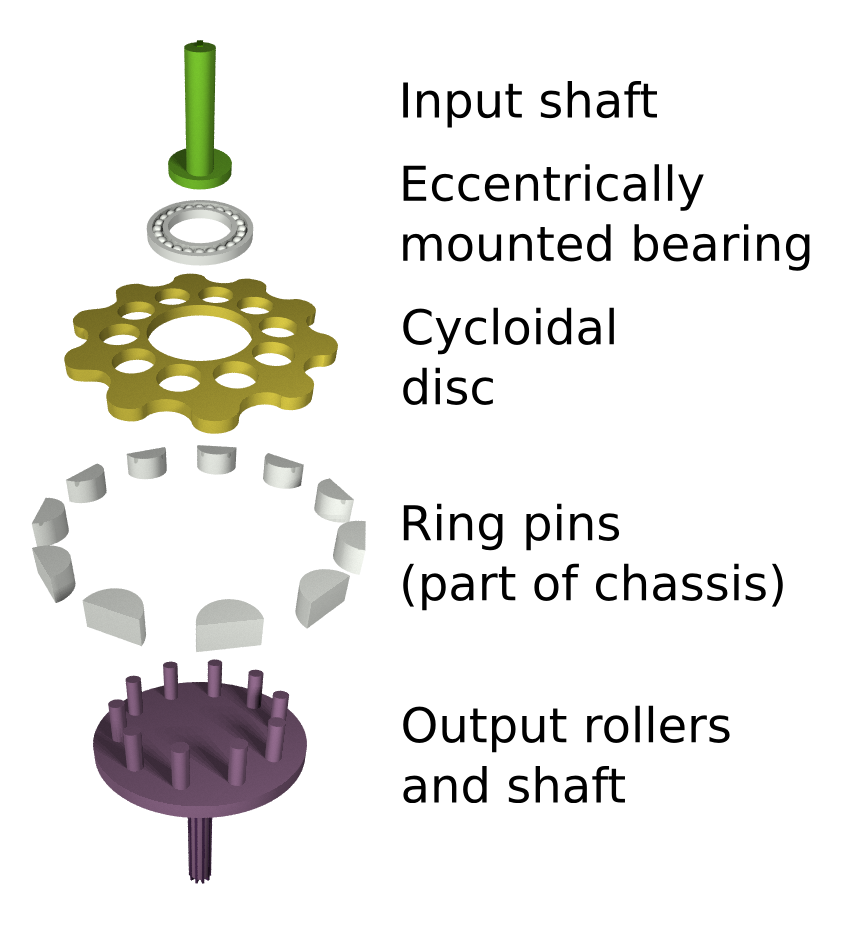
\includegraphics[width=0.60\linewidth]{images/Cycloidal_drive_parts}
    \caption{Simple rendering of the key elements that create a cycloidal drive.
   	A drive shaft spins a cycloidal disk via an eccentric circle (green).
   	The cycloid plate (yellow) reacts against the housing pins (gray) to create a counter-rotation, harnessed by the output pins (purple). (Public domain image from \cite{cycloid_cartoon})}
   \label{cycloid_cartoon}
\end{figure}


\subsection{Cycloidal Drive Background}
Cycloidal drives were proposed as early as 1956 by Botsiber and Kingston \cite{1956}.
The premise of this design leverages a plate, referred to as the cycloid plate, with lobes that interact with pins in the housing being spun on an eccentric shaft with a bearing.
The interaction between the eccentric rotation and the lobes pressing between the pins induces a counter-clockwise motion of the plate. This counter-clockwise rotation is harnessed via the interior pins that connect to a concentric plate that acts as the output of the mechanism (seen in Fig \ref{cycloid_cartoon}). A graphic of this motion, Fig \ref{cycloid_motion}, shows how the cycloid moves through a single input revolution causing 1/7 of an output revolution through the output pins. 
The reduction equation (\ref{eq:single_stage_ratio}) gives the overall reduction of the single-stage cycloid where \textit{N\textsubscript{lobes}} is the number of lobes on the cycloid plate and \textit{N\textsubscript{pins}} is the number of pins in the housing. 

\begin{equation} \label{eq:single_stage_ratio}
Q = \frac{N_{lobes}} {N_{pins} - N_{lobes}}
\end{equation}

This geartrain design has been used in industry for high torque, high shock load applications for many years by companies like Nabtesco Motion Control.
However, in many of these applications, many or all of the interacting surfaces like the housing pins and output pins use needle roller bearings to transmit load.
This allows for higher efficiency and load carrying capability, but it also increases mass and volume.
In the robotic industry, groups are striving to reduce the mass and volume of these actuators while still achieving high reduction and load capabilities.
One method for reducing mass is eliminating the rolling elements at the interaction points between the cycloid plate, housing pins, and output pins.
This allows for very compact and strong designs to be considered, but leaves the potential for larger losses and shorter system lifetime.

Many works have been presented on the subject of the theoretical design of these cycloidal drives \cite{on_the_lobe} \cite{hwang_hsieh}, designing with machine tolerances \cite{design_and_application}, contact and stress analysis \cite{li}, and performance characteristics such as torque ripple and backlash \cite{hsieh_traditional} \cite{hsieh_dynamics} as will be presented in Section \ref{design}.
These works lay a solid foundation for a designer, providing the equations and design considerations for a cycloid.
Still, there is a need to present in-use characteristics to support the theoretical calculations and models which has not been met in the current literature.

Theoretical cycloid efficiencies have been reported in the 88-98\% range \cite{Malhorta}, \cite{unified_approach}.
More recently, Sensinger and Lipsey reported experimentally determined efficiencies for fused roller designs (42.3\%) and pin designs (71\%) based on 80 minutes of run-time \cite{cycloid_vs_harmonic}.
The distinction between a fused roller and pin design comes in the design of the housing.
In a fused design, the input pins are machined as part of the housing, and in a pin design, pins are inserted to ride in the housing, allowing relative motion.

Hsieh verified the stress present in the drives in simulation and in-use which demonstrated lower stress levels and torque ripple when using fused rollers \cite{hsieh_dynamics}.
These two results leave an open trade to designers if stress and torque ripple need to be minimized versus maximizing efficiency.

The aim of this work is to utilize a custom cycloid design for a NASA rover application and show the in-use efficiency characteristics over an extended duration test.
The actuator design is presented in Section \ref{design}.
A description of the experimental setup and procedure is provided in Section \ref{methods}.
Finally, the results and analysis of this high torque actuator and its implications are presented and discussed in Section \ref{discussion}.



\section{Cycloid Design}
\label{design}
\begin{table*}[t]
  \vskip0.2cm
  \caption{Designed Duty Cycles for System}
  \label{duty_cycle}
  \begin{center}
    \vskip-0.2cm
    \begin{tabular}{|c||c||c| |c| |c|}
    \hline
    Time Used & Output Torque (Nm) & Output Speed (RPM) & Actuator Torque (Nm) & Actuator Speed (RPM)\\
    \hline
    5\% & 2440 & 6.8 & 554.7 & 33.9\\
    \hline
    20\% & 1627 & 6.8 & 369.8 & 33.9\\
    \hline
    60\% & 542 & 15.3 & 123.3 & 76.3\\
    \hline
    15\% & 135 & 15.3 & 30.8 & 76.3\\
    \hline
    \end{tabular}
  \end{center}
\end{table*}

In 2007 and 2008, NASA developed a manned rover prototype for planetary surfaces for future missions \cite{rover}.
This robotic vehicle is made up of six independent wheel modules, each with their own drive, steering, and both active and passive suspension.
In 2014, a new prototype wheel module was designed and created to analyze potential technologies that could be used in these applications.
In the new design layout, it was possible for the drive wheels to counter-rotate against the steering and put large shock loads into the steering system.
These requirements called for a compact package, high load, high shock load, and tolerance of backlash lent themselves to the selection of a cycloidal drive for the steering actuator.
The prototype wheel module layout can be seen in Fig \ref{wheel_module}.

\begin{figure}[t]
   \centering
   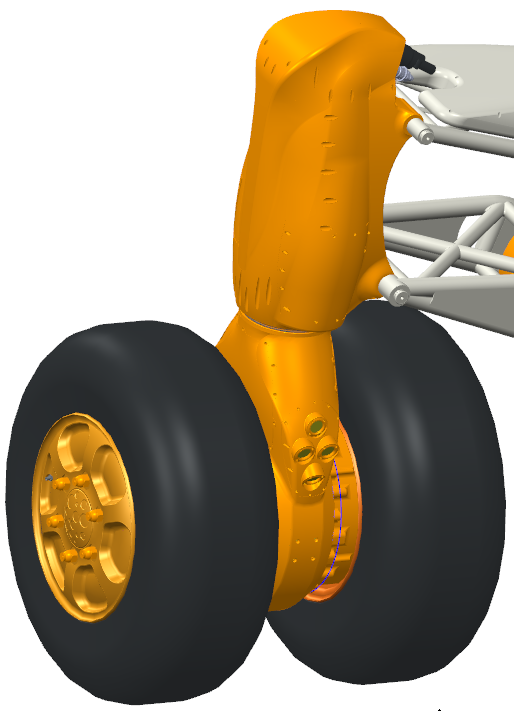
\includegraphics[width=0.40\linewidth]{images/wheel_module_CAD}
   \caption{CAD model of rover wheel module prototype.
   Suspension arms hold the steering column.
   Each wheel has an in-wheel drive motor.}
   \label{wheel_module}
\end{figure}

Based on the load cases, the actuator was required to output a stall torque of 2,440 Nm (1800 ft-lb) with a max output speed of 1.57 rad/s (90 deg/s) at 1,626 Nm (1200 ft-lb).
The required torque/speed data points are presented in Table \ref{duty_cycle} with an assumed efficiency of 88\% chosen based on the available literature.
The actuator layout for the vehicle placed the motor and cycloid off center of the steering axis with an additional 5:1 reduction into the steering column, thus decreasing the torque needed for the cycloid output, but increasing the potential shock loading.

Many sources have laid out the design parameters for these drives and these were used as the design basis of the cycloid.
The equations presented by Shin and Kwon \cite{on_the_lobe} were used as the mathematical definition of the cycloid profile.

\begin{figure}[!b]
	\centering
	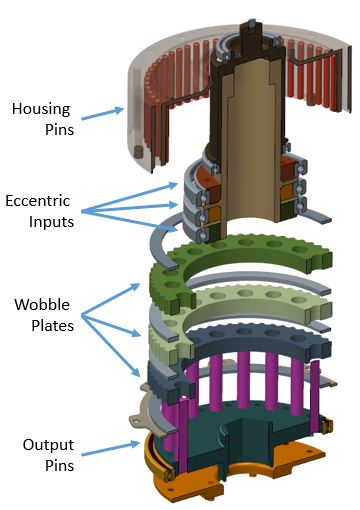
\includegraphics[width=0.7\linewidth]{images/exploded_labeled}
	\caption{Exploded view of the cycloidal reducer.
		Three wobble plates are driven by the input shaft with 120\textdegree\ offsets.
		The ring pins are are free pins inserted in the housing.
		The output has pins run through all three wobble plates to harness the counter-rotation for the drive output.}
	\label{cycloid_exploded}
\end{figure}

Using both the formula for the reduction in diameter of the cycloid disk to account for machine tolerances \cite{machine_design} \cite{design_and_application} as well as Ye et al.'s formula for calculating the limit of undercutting \cite{ye}, the allowable sizes of the profiles and pins can be determined.
Sensinger \cite{unified_approach} laid out simple equations for calculating stress on the lobes and pins that has been further modeled and studied by others. Using these equations, the forces on the cam, bearings, and cycloid plates were calculated. 
The stress calculations and trading of overall size and ratio led to a necessary plate thickness of 2.38cm (0.9375in).
Instead of a single large plate, three wobble plates were selected to split the load on the central input shaft across three bearings as well as to build in natural balance for the actuator.
If a single plate is used, a counterbalance must be added to avoid substantial vibration.
In this case, the three plates were offset 120\textdegree\ to balance these loads and vibration.
This adds stack height to the system to allow separation between the plates.
This arrangement allows the design loads to be able to be handled by the system.
The exploded view of this design can be seen in Fig \ref{cycloid_exploded}.

The actuator uses a Parker Frameless Kit Motor, model K089200-7Y with no hall effect sensors and is commutated using a Renishaw RM-44 magnetic incremental and absolute position sensor.
The final reduction is 59:1 followed by the final 5:1 output gear.
The system is commutated using the delta hysteresis commutation scheme and PI velocity control was implemented to maintain constant motor speeds \cite{electric_machines}.



\section{Experimental Methods}
\label{methods}
\begin{figure}[!b]
   \centering
   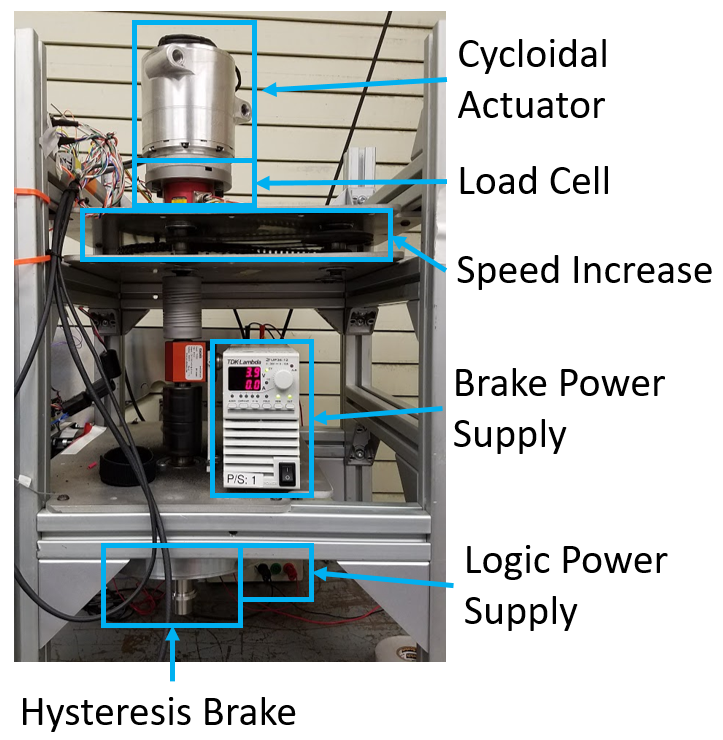
\includegraphics[width=0.75\linewidth]{images/test_stand}
   \caption{Experimental Test Setup.
   The cycloid actuator is mounted to structure via the load cell.
   There is a speed increase so the brake can generate enough torque on the system.
   Not pictured is the controlling computer, motor driver, and high voltage supply.}
   \label{test_setup}
\end{figure}

The authors sought to experimentally determine and compare the cycloidal drive in-use efficiency results to the published performance data for a comparable harmonic drive.The test setup is shown in Fig \ref{test_setup}.
The actuator is mounted directly to a Futek TF600 5000inlb load cell to measure direct output torque of the actuator.
This is read through a load cell conversion board into the motor driver.
A verification of torque readings was completed using a calibrated torque wrench to ensure accuracy of the conversion.
The motor output runs through a 36:1 (TODO) speed increase via three chain stages that then inputs into a Magtrol HB-1750 hysteresis brake that is powered using a separate 24V Lambda-TDK power supply controlled by the computer.
The motor is driven with a custom motor driver powered from a 12V Lambda-TDK power supply for logic power, and a 300V, 5A TDK-Lambda power supply for motor power.
The motor is commutated using the incremental encoder and an index pulse and is reading the RMS phase current, motor and bridge temperatures with thermistors, motor velocity, and the torque measurement from the custom conversion board.
These values are then streamed to a controlling computer that is also monitoring the high voltage supply and recording voltage and current to determine input power to the system.

Due to the tightly integrated actuator design, the motor and cycloid cannot be separated to purely isolate the losses in the cycloid.
The efficiency map of the motor over its torque and speed range was provided by Parker Motors.
For calculation purposes, this table is used as a lookup table for efficiency of the motor given the current motor velocity and rms input current.
While this does generate a level of uncertainty in the data, these motors are mass manufactured and defects are assumed to be small.
Therefore, the error in the motor efficiency map is assumed to be small and would not influence the perceived trends and results.
The efficiency losses in the motor driver can be characterized primarily by the TODO -- switching electronics and which are rated as 97\% efficient in this voltage and current range -- TODO.

\begin{figure}[!b]
   \centering
   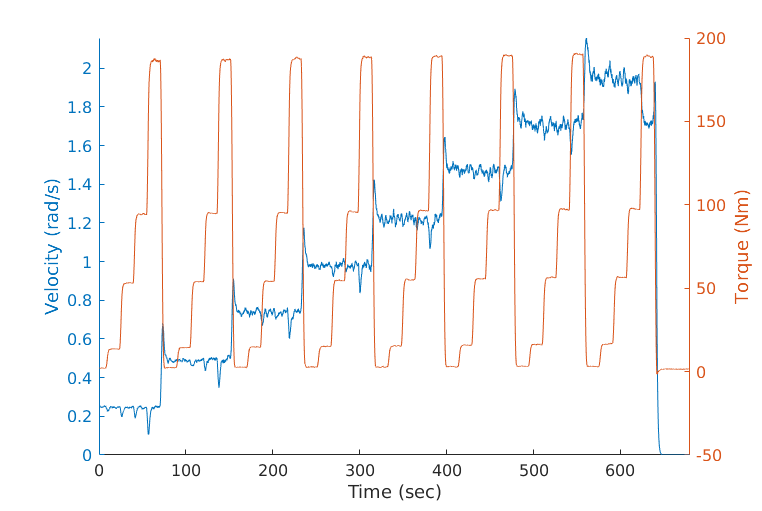
\includegraphics[width=\linewidth]{images/eff_test_profile_v4}
   \caption{Testing profile for efficiency.
   At each speed step, torque is ramped up through five different levels, then the speed is increased.
   At the last step, the maximum of the supply was reached so motor velocity dropped.}
   \label{eff_profile}
\end{figure}

The system was tested in two separate ways, an efficiency cycle and a long term drive cycle.
The efficiency cycle test was run after the long term drive cycle to ensure steady state performance before cycling through a set of velocities and torques.
The actuator is subjected to eight velocity steps increasing 0.25 rad/s each time.
In each velocity step, the torque is ramped up and maintained for 15 seconds at values of 1Nm, 15Nm, 52Nm, 94Nm, and 189Nm.
This testing profile can be seen in Fig \ref{eff_profile}.
The long term drive cycle was run continuously each day for 6 to 12 hours with the duty cycles shown in Table \ref{table_2}.
The total runtime of the system not including the initial checkout and verification of the actuator has been 111 hours.

\begin{table}[h]
  \caption{Long Run Drive Cycle}
  \label{table_2}
  \begin{center}
    \begin{tabular}{|c||c||c|}
    \hline
    Time (s) & Velocity (rad/s) & Torque (Nm)\\
    \hline
    150 & 1.0 & 0.0\\
    \hline
    150 & -1.0 & 0.0\\
    \hline
    60 & 0.5 & 26.0\\
    \hline
    60 & -0.5 & 26.0\\
    \hline
    150 & 1.5 & 10.0\\
    \hline
    150 & -1.5 & 10.0\\
    \hline
    30 & 1.0 & 50.0\\
    \hline
    30 & -1.0 & 50.0\\
    \hline
    300 & 0.5 & 18.0\\
    \hline
    300 & -0.5 & 18.0\\
    \hline
    \end{tabular}
  \end{center}
\end{table}

It should be noted that the actuator was used briefly in the robot validation after initial development and construction of the prototype wheel module.
The total time of use was approximately three hours.
Afterwards, it was removed from the wheel module and subjected to the individual testing that is discussed in this work.
The motor has a continuous current rating of 4.3 A\textsubscript{rms} and a peak rating of 15A\textsubscript{rms}.
The actuator was designed to be fluid cooled to allow operations above the continuous values, but this could not be achieved during testing.
For long duration testing, the torque values were decreased to avoid thermal issues.
The motor was tested to approximately 6A\textsubscript{rms} during efficiency testing due to the limit of the power supply.
Also, the motor driver's rated limits are 150V, therefore the actuator's maximum rated speeds could not be attained.
The nominal cycle of the actuator as seen in Fig \ref{duty_cycle} is still achievable and has been tested.

\begin{figure*}[t]
   \centering
   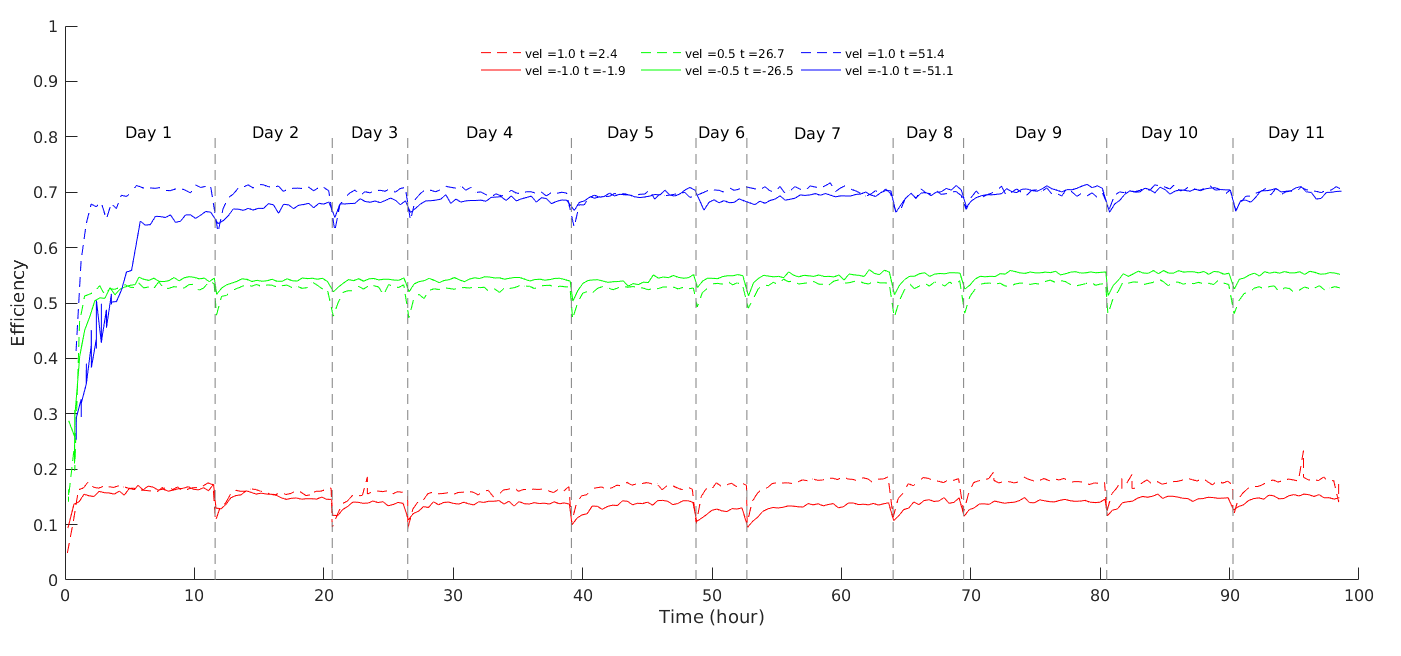
\includegraphics[width=\linewidth]{images/long_run_plot_v4}
   \caption{Efficiency over time for three different speed/torque profiles during the drive cycle.
   The forward motion can be seen with the dotted line, reverse with the solid line.
   At the onset of testing, visible efficiency gains are made.
   As each day begins, there is a clear warm-up period before steady state.
   TODO: add a line for start of each day}
   \label{long_run}
\end{figure*}



\section{Results}
\label{results}

\begin{figure*}[t]
   \centering
   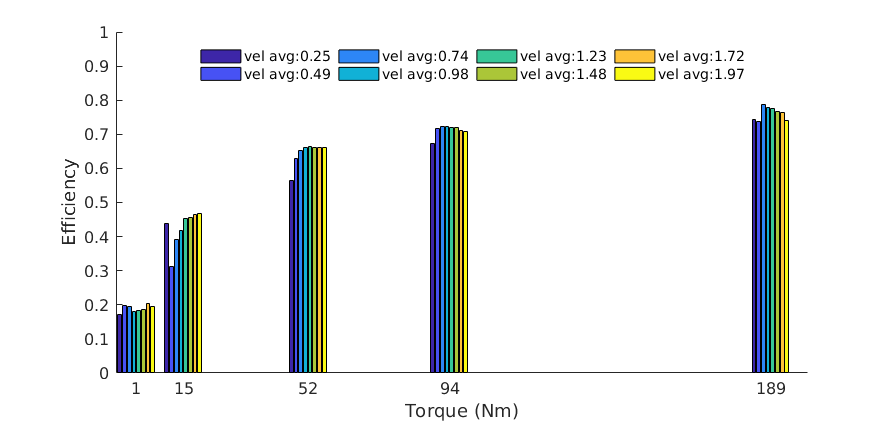
\includegraphics[width=0.8\linewidth]{images/eff_test_bar_plot_v3}
   \caption{Grouping of average efficiencies at each torque step.
   Efficiency depends heavily on torque, and slightly on speed.}
   \label{eff_results}
\end{figure*}

Duty cycle testing was first performed on the actuator.
These tests were done at lower torques to prevent the motor from overheating to allow extended duration testing.
The total test time prior to these duty cycle tests was approximately 5.2 hours to bring up and check out the actuator testbed system.
Once this checkout was complete, the 100 hours of duty cycle testing were conducted the course of 11 days with the drive cycle discussed in Section \ref{methods}.
Three of the torque/speed combinations in forward and reverse are plotted on Fig \ref{long_run} to show the general characteristic trends seen in actuator performance.

After this duty cycle testing to ensure the actuator had sufficiently broken-in and achieved steady state performance, the pure efficiency cycles were run.
As discussed in Section \ref{methods}, a profile of speeds and torques were run on the actuator to show the relationship between speed, torque, and efficiency.
An example of this profile can be seen in Fig \ref{eff_profile}.
This profile was run three times and the results at each torque and speed combination were averaged (see Fig \ref{eff_results}.


\section{Discussion}
\label{discussion}
\todo[inline]{Removed wording about comparing to a planetary, will change the figure when I get to the computer that has the figure tomorrow} 

The efficiency of the system is dependent on the torque through the gearbox as shown in Fig \ref{eff_results}.
This contradicts previous studies that suggested that cycloidal drives have a constant efficiency across the torque range.
There is also a much less pronounced relationship between the velocity and the cycloid efficiency that can be noted in the torque bands.
This result suggests that the cycloid efficiency behaves similarly to a typical reduction like a planetary or a harmonic drive in its increase of efficiency as torque increases. 
A comparison of the tested cycloidal drive and a harmonic drive can be seen in Fig \ref{eff_comp}.
The figure shows the efficiency for a harmonic drive CSF-45-50-2UH-LW \cite{harmonic_sheet} which has a comparable ratio and torque capability to the tested cycloid and weighs 5.1kg.
If backlash is acceptable in a system, a cycloidal drive can provide similar or better efficiency profiles to a harmonic drive while providing a potential 2x increase in specific torque (Nm/kg).

\begin{figure}[t]
   \centering
   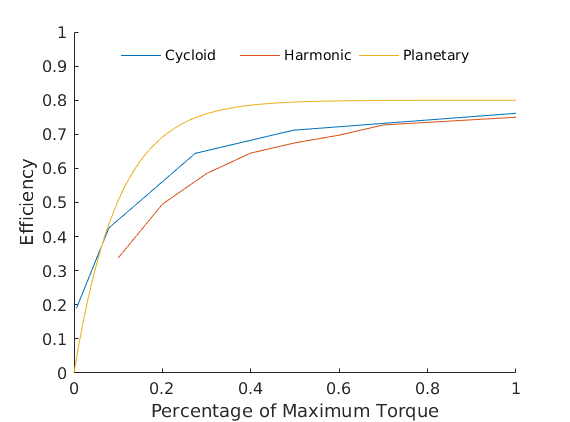
\includegraphics[width=\linewidth]{images/eff_comp_v3}
   \caption{Comparison of efficiency over maximum torque rating of the tested cycloid and a comparable harmonic drive.
   The cycloid exhibits the same efficiency increase over torque range and has a comparable and slightly higher efficiency than the harmonic. TODO: Replace with version not including planetary}
   \label{eff_comp}
\end{figure}

\todo[inline]{added wording and figure about the wear in to support claims} 

There was a substantial break-in time for the actuator before steady state results were achieved (see Fig \ref{long_run}).
In the high torque case, specifically in the reverse direction, there was an approximately linear increase in efficiency over the course of the first seven hours of duty cycle testing.
This testing began after a minimum of five hours of run time spread out through many short sessions while getting the test system running.
The large increase in efficiency can be noted in the other lower torque profiles as well, starting well below their final steady state values.
The authors theorize that this is due to break-in of the manufactured parts required because of machining inaccuracies.
Due to the complex interaction required of the trochoidal motion profile, slight manufacturing deficiencies could cause build-ups of stress and loss in particular points on the drive.
It would make sense that these could manifest in one direction and not the other if a lobe was misshapen on the trailing edge in one direction, it would be the lead edge in the other direction, causing the additional loss.
Through the first hours of testing, these materials likely wore in to each other until the contact was smooth, resulting in the more readily achieved steady state efficiencies in subsequent hours of testing.
This wear in can be seen on the lobes of the cycloid plate observed after testing in Fig \ref{cycloid_plate}.

\begin{figure}[t]
	\centering
	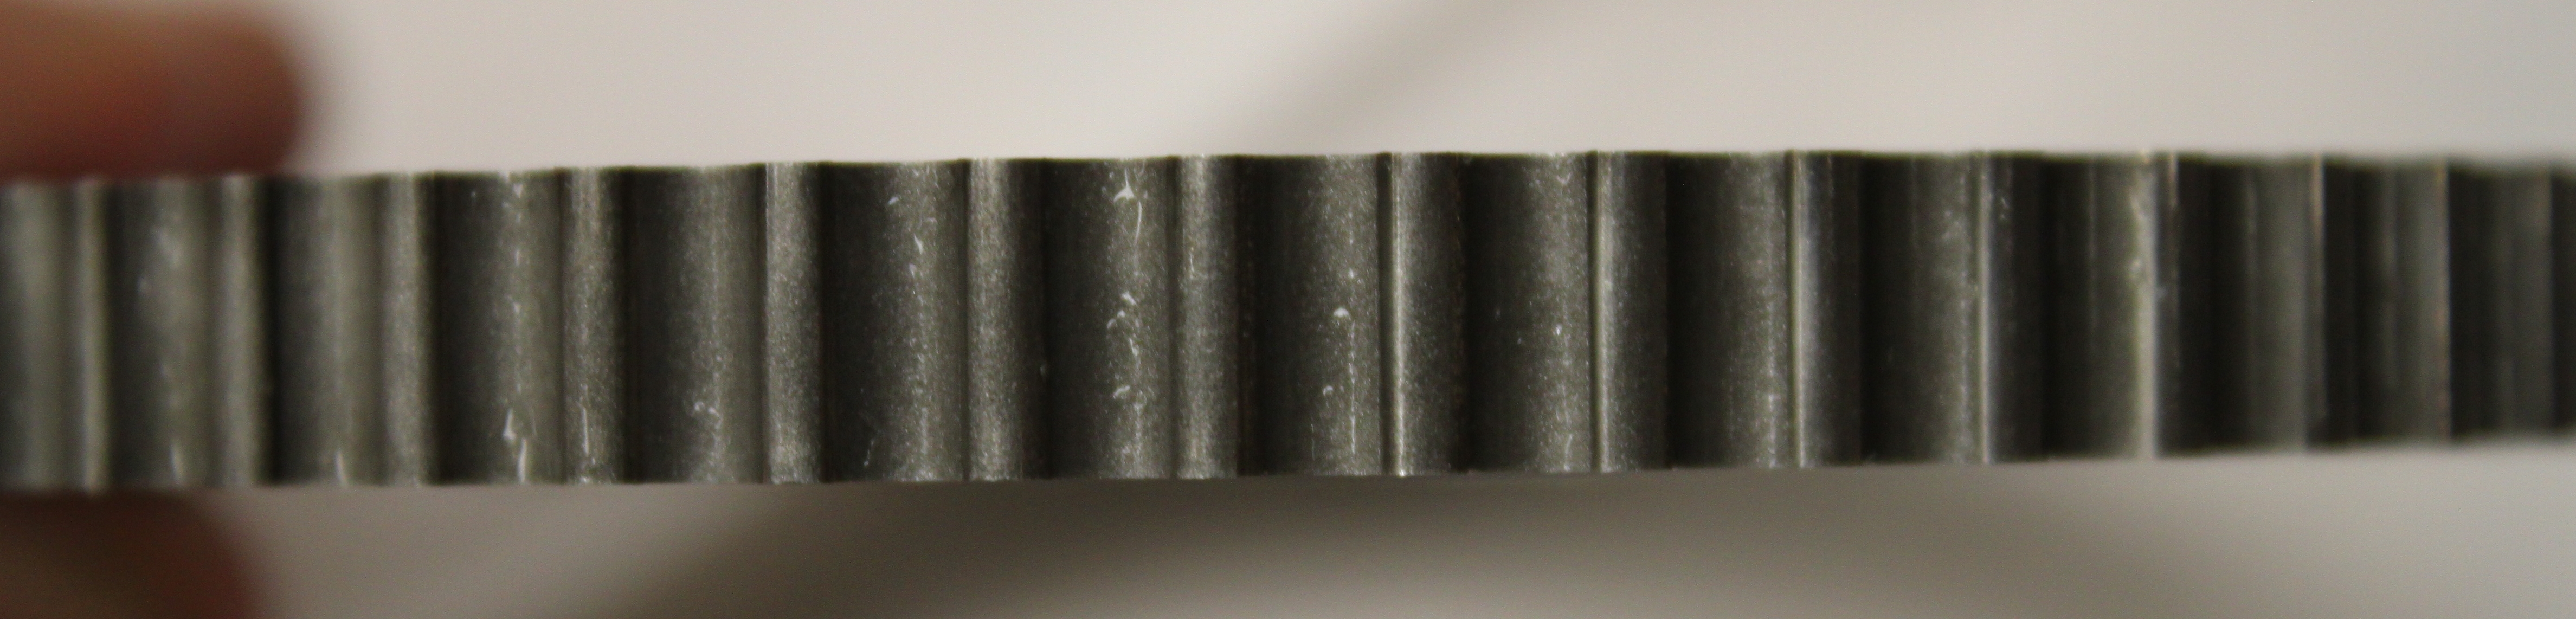
\includegraphics[width=\linewidth]{images/cycloid_plate}
	\caption{Profile of one of the cycloid plates. Each lobe shows smoothing along the convex portion of the lobe and no wear along the concave portion. The wear is also uniform around the profile, showing relatively even load distribution around the profile during operation. This slight wear indicates that wear was occurring and could have smoothed defects to increase efficiency during break-in.}
	\label{cycloid_plate}
\end{figure}

Additionally, there is a marked improvement over the first 30 minutes of runtime in the efficiency of the system.
This is likely due to the grease and heat in the system.
The gearbox is greased with Lucas Oil Red'N'Tacky which has a viscosity index of 86 min.
This was chosen because it is designed for high loads for extended periods of time in gear and sliding surface applications, as well as ease of use for Earth testing and verification.
Therefore, during the warm-up period as the actuator temperature increases, the viscosity decrease is likely enough to cause a notable increase in efficiency of the system.
The authors leave the study of a lower viscosity grease's effect on performance, as well as grease suitable for vacuum, for future work.



\section{Conclusion}
\label{conclusion}
The aim of this work was to determine the in-use characteristics of a cycloidal drive designed for a robotic application through an extended break-in test and efficiency testing.
Through the work, this study demonstrates a cycloidal actuator with a ratio of 59:1 and three phased cycloid disks that achieves a maximum efficiency of 80\% and does not show a constant efficiency through its torque profile as suggested by previous sources.
This research shows that these drives efficiencies behave very similarly to other typical reduction drives for similar applications like Harmonic Drives and Planetary gears.
This actuator compares closely to its Harmonic Drive counterpart in efficiency performance.
If backlash is acceptable in the system, a cycloidal drive has the distinct advantage of being customized into the housing using simple manufacturing techniques allowing tighter integration into a robotic system as well as a potential 2x specific torque gain.
While the efficiency and load capacity may be higher when using rolling elements for the input and output pins, this research shows that efficiencies in a similar range to other high reduction drives can be achieved when these heavy and large rolling elements are not used.
An item of interest that has not been characterized by the community is the lifetime characteristics of this cycloid design style and this is left by the authors for future work.
Cycloidal drives of this design style are quite comparable to similar use-case drives and should be considered in high reduction applications.



\section{Acknowledgements}
\label{acknowledgements}
The authors would like to thank the original actuator designer, Mason Markee, for his support in the testing and research of this system.  

\bibliographystyle{IEEEtran}
\bibliography{Cycloid_ICRA_Bib}

\end{document}
